\chapter{Data Acquisition and Content Intelligence}
\label{ch:data-pipeline}

The pipeline codebase (\texttt{app/}) is the single point of entry through which every piece of content (a paper, a code release, a video, a government filing, a funding announcement) enters AI Compass. This chapter documents the full path an item travels from external source to a scored, embedded, clustered row in the shared database: how sources are registered and dispatched, how a user-submitted feed is screened before it is trusted, how one language-model call produces the structured intelligence attached to every item, how a deterministic quality score is computed, and how near-duplicate coverage of the same real-world story is detected and merged. Every mechanism described here is a design choice made under the project's governing principle stated in Chapter~1 (\emph{ingest once, personalize later}), so none of the computation in this chapter is user-specific; it runs exactly once per item, globally, regardless of how many users eventually see the result.

\section{Source Registry and Ingestion Adapters}
\label{sec:source-registry}

AI Compass ingests content through a \texttt{sources} database table that currently holds 16 rows. Of these, 9 are dispatched through an adapter registry keyed by a \texttt{source.key} string: \texttt{arxiv}, \texttt{github\_release}, \texttt{youtube}, \texttt{reddit}, \texttt{government\_us}, \texttt{government\_uk}, \texttt{government\_nist}, \texttt{funding\_crunchbase}, and \texttt{huggingface\_model}. A further 2 rows (\texttt{blog\_openai} and \texttt{blog\_anthropic}) are legacy stubs: they exist only as foreign-key anchors so that historical articles retain a valid \texttt{source\_id}, but the registry never dispatches them, because the actual OpenAI and Anthropic blog scraping is performed by a separate, hardcoded \texttt{BlogScraper} that bypasses the registry entirely. The remaining rows are sources that individual users submitted through the product and that passed the relevance gate described in Section~\ref{sec:relevance-gate}.

Every registry-dispatched source is handled through a common adapter interface: an abstract \texttt{BaseScraper} base class defining the scrape-and-persist contract, behind which sit two families of concrete implementation. The first is a single, generic, configuration-driven \texttt{RssFeedScraper} that reads a feed URL and a small set of parsing hints from the source's own database row, so adding a new pure-RSS source requires zero new code: only a new row in \texttt{sources}. The second family consists of five bespoke \texttt{BaseScraper} subclasses, written where the source exposes a structured JSON or REST API rather than an RSS feed and therefore cannot be handled generically: the arXiv API, the GitHub Releases API, the YouTube Data API (paired with transcript retrieval, Chapter~8), the Federal Register API, and the Hugging Face Hub API. This is a deliberate cost-of-extension trade-off: the common RSS case is free to add, while sources whose data model genuinely differs earn their own adapter rather than being force-fitted into a generic one.

\section{User-Submitted Source Screening}
\label{sec:relevance-gate}

Users can propose their own sources, which raises an obvious risk: an unscreened submission could flood the shared content pool with material unrelated to AI, degrading the corpus for every other user. AI Compass gates every user-submitted source behind an automated relevance check before it is admitted into the registry-eligible pool. A deliberate, disclosed design decision governs how this check works: it is \emph{not} a generative-AI judgment call. Routing every submission through a large language model would add both latency and per-submission cost to a request path that a Django worker is synchronously blocked on, for a decision that does not require language understanding at the level an LLM provides.

Instead, the gate is a cheap, deterministic, embedding-similarity heuristic. The candidate feed's most recent items are embedded (using the same embedding model described in Section~\ref{sec:schema}), and the mean cosine similarity between those item embeddings and a corpus centroid is computed, where the centroid is the mean embedding of a 500-row random sample drawn from the existing \texttt{embeddings} table. Let $\bar{s}$ denote this mean similarity. The decision rule is:
\begin{equation}
\label{eq:relevance-gate}
\text{decision}(\bar{s}) =
\begin{cases}
\text{accept} & \text{if } \bar{s} \geq 0.30 \\[2pt]
\text{reject} & \text{if } \bar{s} \leq 0.12 \\[2pt]
\text{keyword fallback} & \text{otherwise}
\end{cases}
\end{equation}
Submissions whose similarity falls in the gray zone between the two thresholds are resolved by a secondary, equally non-generative heuristic that measures the density of AI-related keywords in the candidate items, rather than being defaulted to either outcome. The gate is intentionally conservative at both ends and defers only the ambiguous middle to a second cheap signal, keeping the entire check free of any per-submission LLM inference.

\section{Content Enrichment}
\label{sec:enrichment}

Once an item is ingested and deduplicated (Section~\ref{sec:schema}), it is enriched exactly once by a single structured LLM call on Groq's cheapest tier, \texttt{llama-3.1-8b-instant}, returning a Pydantic-validated output containing a summary, controlled-vocabulary topics, named entities, a \texttt{content\_category} label, a \texttt{technical\_depth} rating (1--5), key points, technical details, a business angle, and a ``why it matters'' statement. This deliberately replaces what would otherwise be four or five separate per-item calls (summarization, topic tagging, entity extraction, category classification, business-relevance) with one round trip: since enrichment runs over every ingested item, not per user, this multiplicative saving in latency and cost is the entire justification.

Because the output is machine-generated and only schema-validated, defensive validation applies rather than trusting it outright: an invalid \texttt{content\_category} falls back to \texttt{"other"}, and any entity or topic failing validation against the controlled vocabulary (Section~\ref{sec:taxonomy}) is silently dropped, never invented. A disclosed limitation: content is truncated to its first \texttt{content[:10000]} characters before the call, so long articles and transcripts are only partially seen, mitigated only for long video via Chapter~8's map-reduce mechanism, while ordinary long articles remain subject to the ceiling.

\section{Quality Scoring}
\label{sec:quality-score}

Independently of enrichment, every item receives a deterministic content-quality score, computed by a fully transparent, project-specific formula rather than a learned model. This score is intentionally not drawn from prior recommender-systems literature; it is an AI Compass project-specific formulation, designed to reward exactly the properties that make an item usable downstream (successfully enriched, substantive in length, entity- and topic-rich, and recent):
\begin{equation}
\label{eq:quality-score}
\begin{split}
\text{score} = {}& 0.30\,\mathbb{1}[\text{enriched}] \;+\; 0.20\,\text{length\_score} \;+\; 0.15\,\min\!\left(1,\tfrac{\text{entity\_count}}{5}\right) \\
& {}+\; 0.15\,\min\!\left(1,\tfrac{\text{topic\_count}}{3}\right) \;+\; 0.20\,\text{freshness}
\end{split}
\end{equation}
where $\mathbb{1}[\text{enriched}]$ is 1 if the item has a valid enrichment record and 0 otherwise, \text{entity\_count} and \text{topic\_count} are the number of validated entities and topics attached to the item, and the two component terms are themselves defined as
\begin{equation}
\label{eq:quality-components}
\text{length\_score} = \min\!\left(1,\ \frac{\ln(1+\text{content\_length})}{\ln(1+5000)}\right), \qquad
\text{freshness} = \exp\!\left(-\frac{\text{age\_days}}{14}\right).
\end{equation}
The logarithmic length term rewards substantive content while saturating near 5,000 characters so that arbitrarily long items are not rewarded without bound; the freshness term is an exponential decay with a 14-day half-life-like constant, so a score computed today already discounts an item that was fresh a month ago. This score is stored per item and is not itself a ranking decision; it is one of the five weighted signals consumed by the personalized ranking formula presented in Chapter~6, where it enters as the \texttt{quality} term.

\section{Taxonomy and Named-Entity Extraction}
\label{sec:taxonomy}

AI Compass classifies content along two structurally different axes. The first is a fixed, controlled taxonomy of exactly 27 topic slugs, curated so that every enrichment call assigns topics only from this closed vocabulary rather than free text. Of these 27 slugs, 15 overlap exactly with the vocabulary exposed to users during onboarding as selectable \texttt{Interest} chips; the remaining 12 are content-classification-only topics, judged too technical or too granular to present as a user-facing preference (for example, distinctions useful for indexing research content but not meaningful as an onboarding choice). This split means the taxonomy serves two audiences at once from a single source of truth: the classification layer that tags every item, and the narrower onboarding vocabulary that a user actually sees.

The second axis is named-entity extraction, which is deliberately open-ended rather than drawn from a fixed list. Entities fall into four types (company, model, person, and technology) and are deduplicated within a type by exact name match, i.e. by the pair (name, entity\_type). This is a disclosed limitation rather than an oversight: because deduplication is purely lexical, two spellings of the same real-world entity, such as "OpenAI" and "Open AI," can coexist as distinct entity rows rather than being merged into one canonical record. Resolving this would require an entity-canonicalization step (for instance, a second embedding-similarity pass over entity names, or a curated alias table) that AI Compass does not currently implement; the trade-off accepted here is that entity extraction stays simple and cheap, at the cost of occasional near-duplicate entities that a future canonicalization pass would need to merge.

\section{Near-Duplicate Clustering}
\label{sec:clustering}

The same real-world event is frequently covered by multiple outlets (a model release reported by both a GitHub changelog and several downstream blog posts, for instance). AI Compass detects this kind of near-duplicate coverage through a purpose-built clustering step, run on a schedule as part of every full pipeline pass rather than incrementally. The mechanism is not a clustering library; it is a hand-rolled Union-Find (disjoint-set) data structure~\cite{tarjan1975unionfind} applied over a k-nearest-neighbor similarity graph built with pgvector. For each embedded item, its top-8 nearest neighbors are retrieved by cosine similarity, and an edge is kept between two items only when their similarity is at or above 0.92; connected components in the resulting graph become clusters. The code's own comments are explicit that this targets near-duplicate \emph{story} deduplication (multiple outlets covering one event), not general topical grouping, which is instead served by the taxonomy of Section~\ref{sec:taxonomy}. The pipeline rebuilds cluster membership wholesale on every run rather than incrementally: existing membership rows are discarded and replaced in full each time, trading recomputation cost for mechanism simplicity.

The 0.92 threshold was arrived at empirically. An earlier version used 0.85, at which the templated, near-identical phrasing of Hugging Face model-card summaries collapsed every model-card item in a run into one spurious $\approx$60-item ``mega-cluster,'' an artifact of the template, not any shared real-world story. The fix combined excluding the Hugging Face model-card source from clustering entirely with raising the threshold to 0.92 for every other source, tightening ``near-duplicate'' enough that superficially similar but substantively different items no longer merge. Algorithm~\ref{alg:clustering} summarizes the procedure.

\begin{algorithm}[htbp]
\caption{Near-duplicate story clustering via Union-Find over a k-NN similarity graph}
\label{alg:clustering}
\KwInput{Embedded content items $I$; neighbor count $k=8$; similarity threshold $\tau=0.92$}
\KwOutput{Cluster assignment (or none) for every item in $I$}
Initialize a disjoint-set structure with one singleton set per item in $I$\;
\ForEach{item $i \in I$}{
  $N_i \leftarrow$ top-$k$ nearest neighbors of $i$ by cosine similarity (pgvector ANN query)\;
  \ForEach{neighbor $j \in N_i$}{
    \If{$\cos(i,j) \geq \tau$}{
      \textsc{Union}$(i,j)$ \tcp*[f]{merge the two disjoint sets}
    }
  }
}
components $\leftarrow$ connected components of the disjoint-set structure\;
discard every component of size 1 (no near-duplicate found)\;
delete all existing cluster-membership rows\;
bulk-insert the surviving components as new cluster-membership rows\;
\end{algorithm}

Figure~\ref{fig:screenshot-trending} shows this mechanism as it surfaces to end users: the Trending Stories page groups items by the connected components Algorithm~\ref{alg:clustering} produces, ranking each story by how many distinct sources cover it and letting the user restrict the view to a 48-hour, 7-day, or 30-day recency window.

\begin{figure}[htbp]
\centering
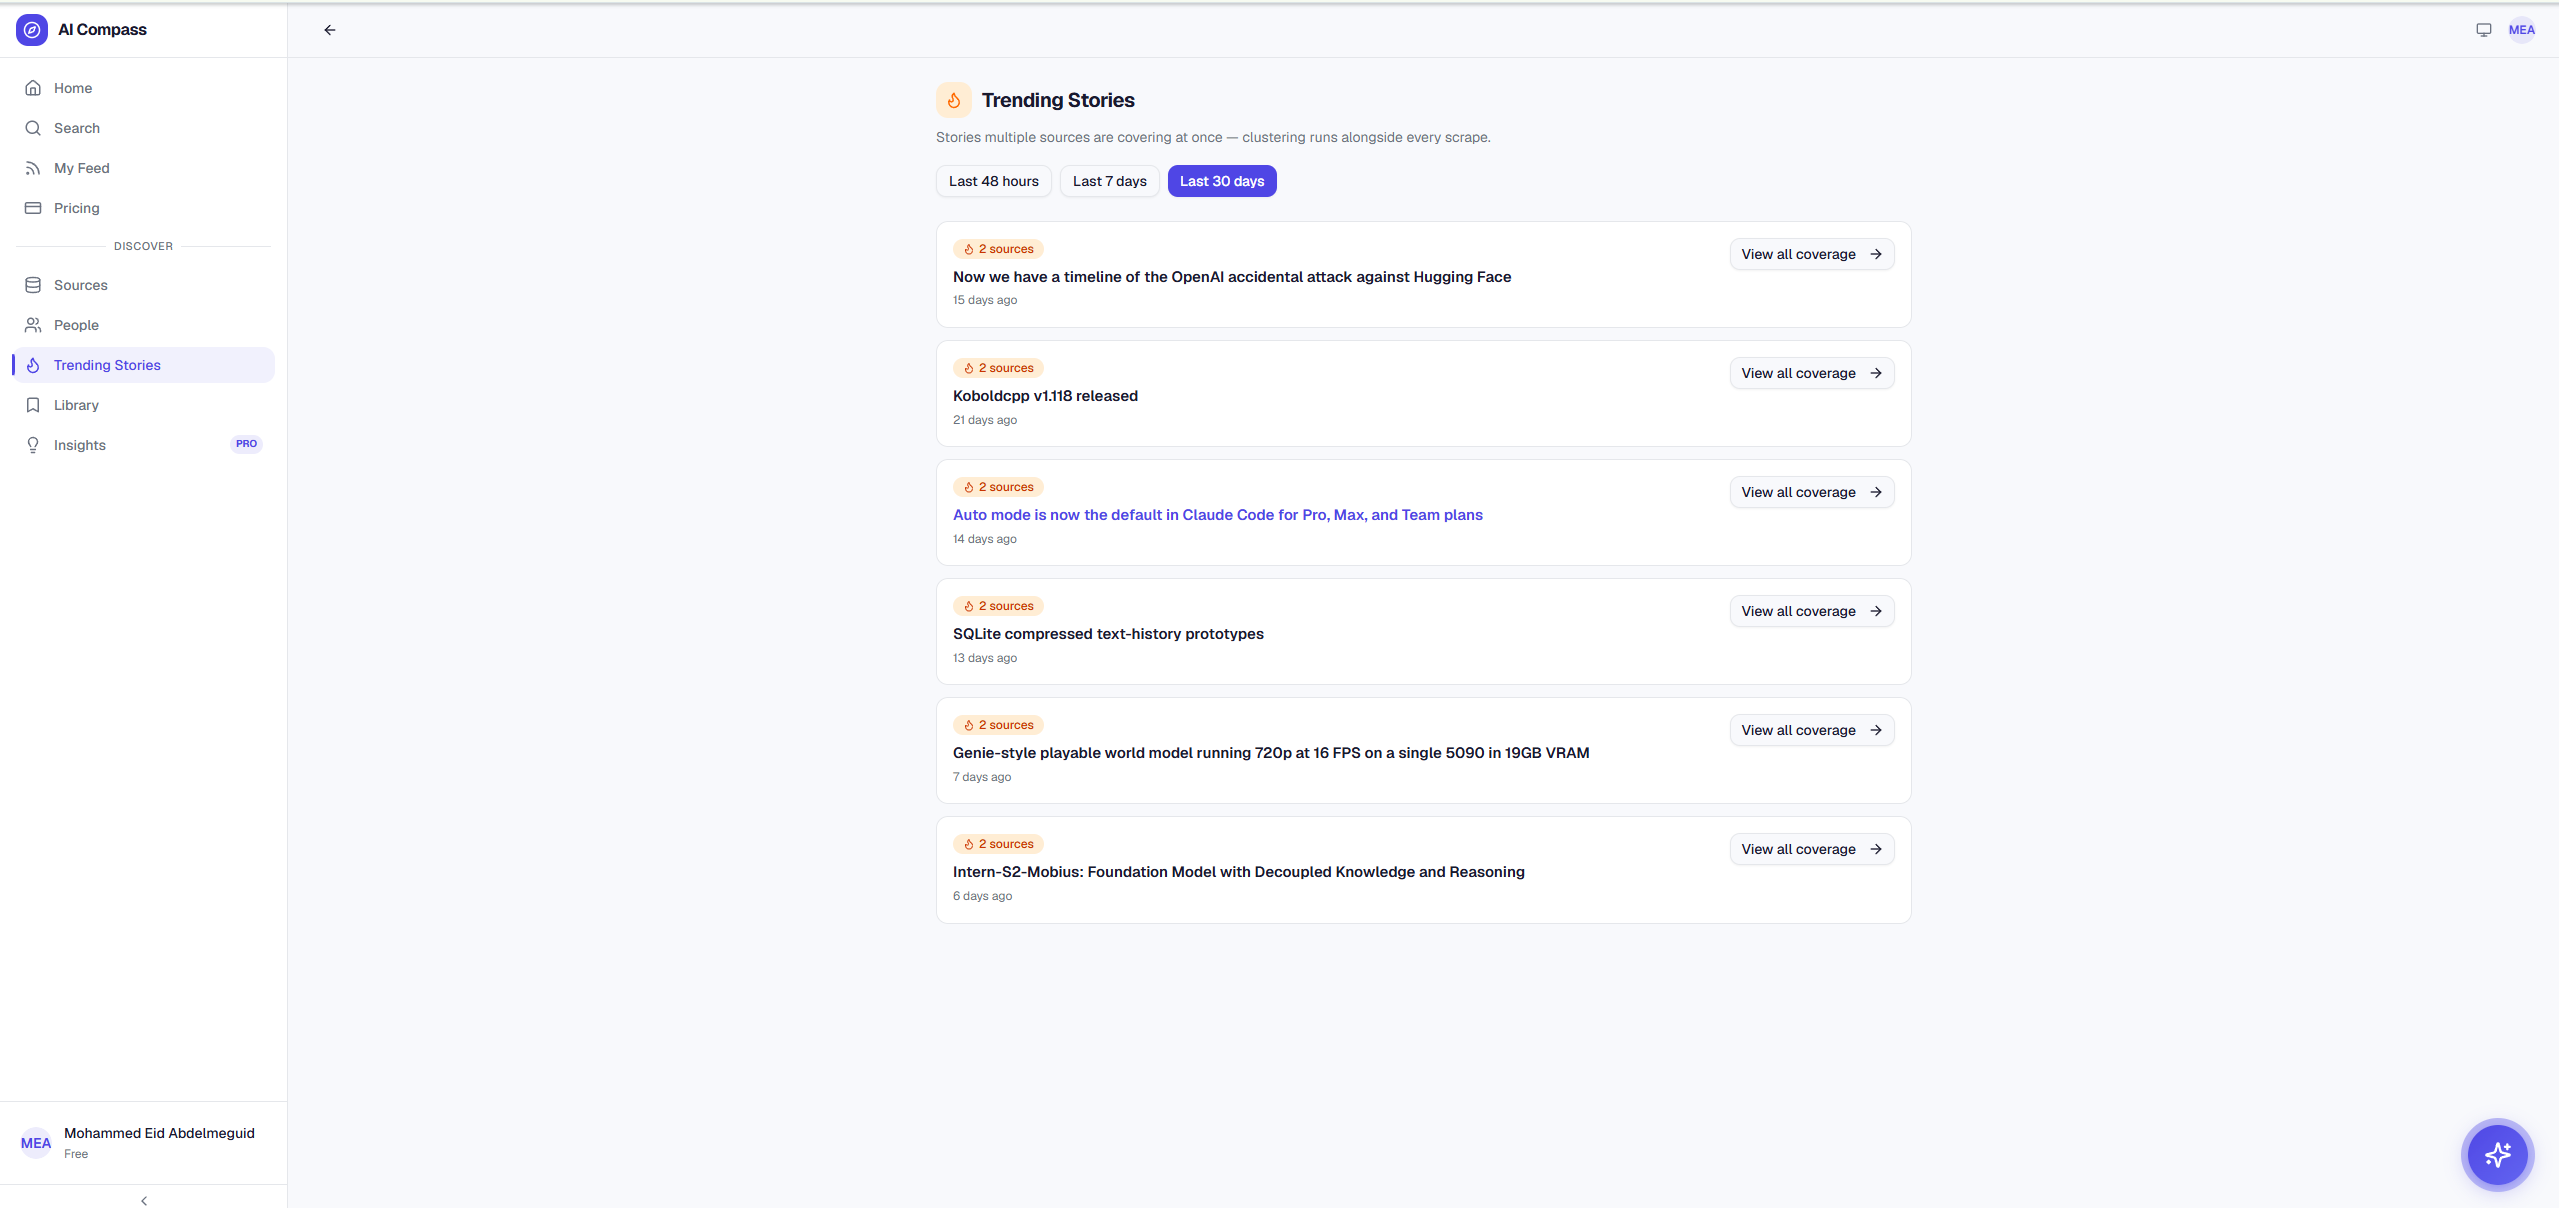
\includegraphics[width=0.85\textwidth]{figures/screenshots/screenshot_trending.png}
\caption{The Trending Stories page, showing near-duplicate story clusters (Section~\ref{sec:clustering}) ranked by the number of distinct sources covering each story, with time-window filters for the last 48 hours, 7 days, and 30 days.}
\label{fig:screenshot-trending}
\end{figure}

\section{Pipeline Data Flow}
\label{sec:pipeline-flow}

Figure~\ref{fig:content-pipeline} lays out the full sequence described in this chapter as a single flow: registry-dispatched and legacy scrapers pull raw items from external sources; ingestion deduplicates and persists them; enrichment attaches the single-call structured intelligence of Section~\ref{sec:enrichment}; embedding computes a vector representation (Section~\ref{sec:schema}); clustering and quality scoring run over the resulting pool; and the passage-level RAG index described in Chapter~7 is populated from the same enriched content. Every stage in this diagram runs once, globally, consistent with the ingest-once-personalize-later principle; none of it is re-triggered by a user viewing content.

\begin{figure}[htbp]
\centering
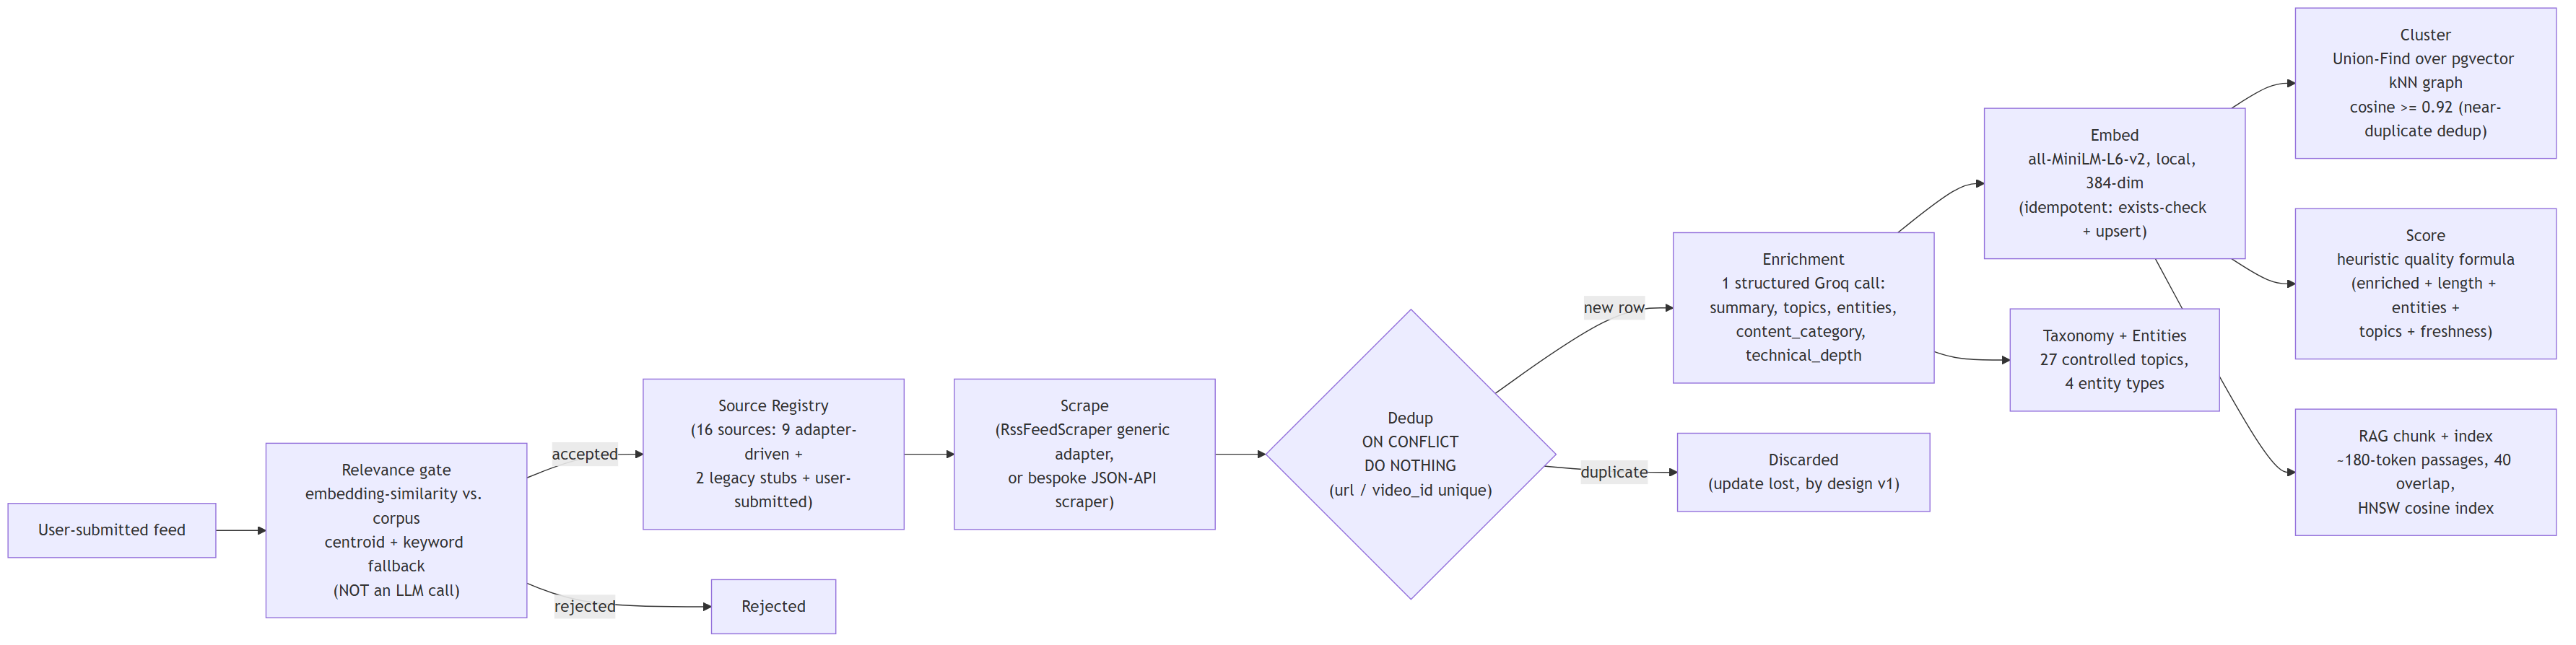
\includegraphics[width=\textwidth,height=0.88\textheight,keepaspectratio]{figures/content_pipeline.png}
\caption{Content ingestion and intelligence pipeline: from source registry through scraping, deduplication, enrichment, embedding, clustering, scoring, and RAG indexing.}
\label{fig:content-pipeline}
\end{figure}

\section{Database Schema}
\label{sec:schema}

The pipeline owns its schema directly through SQLAlchemy, independent of the Django backend's own models (the ownership boundary between the two is formalized in Chapter~4). Figure~\ref{fig:pipeline-schema} shows the pipeline-owned entity-relationship diagram. \texttt{Sources} is the registry table described in Section~\ref{sec:source-registry}; each source's raw items land in \texttt{Articles} or \texttt{YoutubeVideos} depending on content type. Ingestion-time deduplication is enforced at the database level through an \texttt{INSERT ... ON CONFLICT DO NOTHING} clause keyed on a natural unique identifier (the article URL, or the YouTube \texttt{video\_id}), a deliberate v1 design choice that keeps ingestion cheap and idempotent: re-running a scrape never produces duplicate rows. The disclosed cost of this choice is that if a source later republishes a corrected or expanded version of the same URL, that later version is never re-ingested, since the conflict clause silently discards it rather than updating the existing row; this is a genuine limitation of the current design, not an unnoticed bug.

\texttt{ContentEnrichment} stores the structured output of Section~\ref{sec:enrichment}, one row per item, linked polymorphically by a \texttt{(content\_type, content\_id)} pair so the same table serves both articles and videos. \texttt{Embeddings} stores one 384-dimensional vector per item, computed locally with \texttt{all-MiniLM-L6-v2} from the Sentence-BERT / \texttt{sentence-transformers} family~\cite{reimers2019sentencebert,wang2020minilm,sbert_docs}, chosen because it runs locally with no per-embedding API cost, unlike the enrichment LLM call. Every embedding write is idempotent by construction: gated first by an application-level existence check, then independently by a database-level unique constraint on \texttt{(content\_type, content\_id)} enforced through an \texttt{INSERT ... ON CONFLICT DO UPDATE} clause, so duplicate embedding rows are structurally impossible even under a race condition, not merely unlikely. \texttt{RagChunks} is the passage-level index the retrieval-augmented assistant of Chapter~7 queries against; \texttt{ContentClusters} and its membership table record the output of Section~\ref{sec:clustering}; \texttt{ContentScores} stores the quality score of Section~\ref{sec:quality-score}; and \texttt{Entities} / \texttt{TaxonomyTopics} store the two classification axes of Section~\ref{sec:taxonomy}. \texttt{UserRankings}, \texttt{UserAffinities}, and \texttt{UserProfileVectors}, consumed by the ranking mechanism of Chapter~6, were added in a later milestone and are the only tables here that are genuinely per-user rather than global.

\begin{figure}[htbp]
\centering

\includegraphics[width=\textwidth,height=0.88\textheight,keepaspectratio]{figures/pipeline_schema.png}
\caption{Entity-relationship diagram of the pipeline-owned (SQLAlchemy) database schema, including the passage-level RAG index (\texttt{rag\_chunks}) and personalization tables (\texttt{user\_rankings}, \texttt{user\_affinities}, \texttt{user\_profile\_vectors}) added in later milestones.}
\label{fig:pipeline-schema}
\end{figure}

\section{Ingestion Sources Table}
\label{sec:sources-table}

Table~\ref{tab:sources} summarizes the composition of the 16-row \texttt{sources} table, grouped by how each row reaches the content pool: the 9 sources dispatched through the adapter registry, the 2 legacy stub rows, and the remaining user-submitted sources that were admitted through the relevance gate of Section~\ref{sec:relevance-gate}.

\begin{table}[htbp]
\centering
\caption{Composition of the \texttt{sources} registry table (16 rows total).}
\label{tab:sources}
\small
\begin{tabular}{|p{2.3cm}|p{3.4cm}|p{4.4cm}|p{2.6cm}|}
\hline
\textbf{Category} & \textbf{Registry key} & \textbf{Adapter type} & \textbf{Dispatch status} \\
\hline
Research literature & \texttt{arxiv} & Bespoke (arXiv API) & Registry-dispatched \\
\hline
Open-source releases & \texttt{github\_\allowbreak release} & Bespoke (GitHub Releases API) & Registry-dispatched \\
\hline
Long-form video & \texttt{youtube} & Bespoke (YouTube Data API + transcripts) & Registry-dispatched \\
\hline
Developer community & \texttt{reddit} & Generic \texttt{RssFeedScraper} & Registry-dispatched \\
\hline
Government (US) & \texttt{government\_\allowbreak us} & Bespoke (Federal Register API) & Registry-dispatched \\
\hline
Government (UK) & \texttt{government\_\allowbreak uk} & Generic \texttt{RssFeedScraper} & Registry-dispatched \\
\hline
Government (NIST) & \texttt{government\_\allowbreak nist} & Generic \texttt{RssFeedScraper} & Registry-dispatched \\
\hline
Funding \& investment & \texttt{funding\_\allowbreak crunchbase} & Generic \texttt{RssFeedScraper} & Registry-dispatched \\
\hline
Model databases & \texttt{huggingface\_\allowbreak model} & Bespoke (Hugging Face Hub API) & Registry-dispatched \\
\hline
Legacy blog scraping & \texttt{blog\_openai}, \texttt{blog\_\allowbreak anthropic} & Hardcoded \texttt{BlogScraper} & Inert FK-only stubs; bypasses registry \\
\hline
User-submitted & (varies) & Generic \texttt{RssFeedScraper} & Admitted via relevance gate \\
\hline
\end{tabular}
\end{table}

Once admitted, a user-submitted row is scraped through the same generic \texttt{RssFeedScraper} used by any other RSS-based registry source, with no separate code path distinguishing it from one that AI Compass shipped with by default.

Figure~\ref{fig:screenshot-sources} shows the Sources page that exposes Table~\ref{tab:sources}'s registry to the end user: every registry-dispatched source listed with a per-user visibility toggle, the category filter chips corresponding to each row's grouping, and the submission form through which a new user-supplied RSS or YouTube feed enters the relevance gate of Section~\ref{sec:relevance-gate}.

\begin{figure}[htbp]
\centering
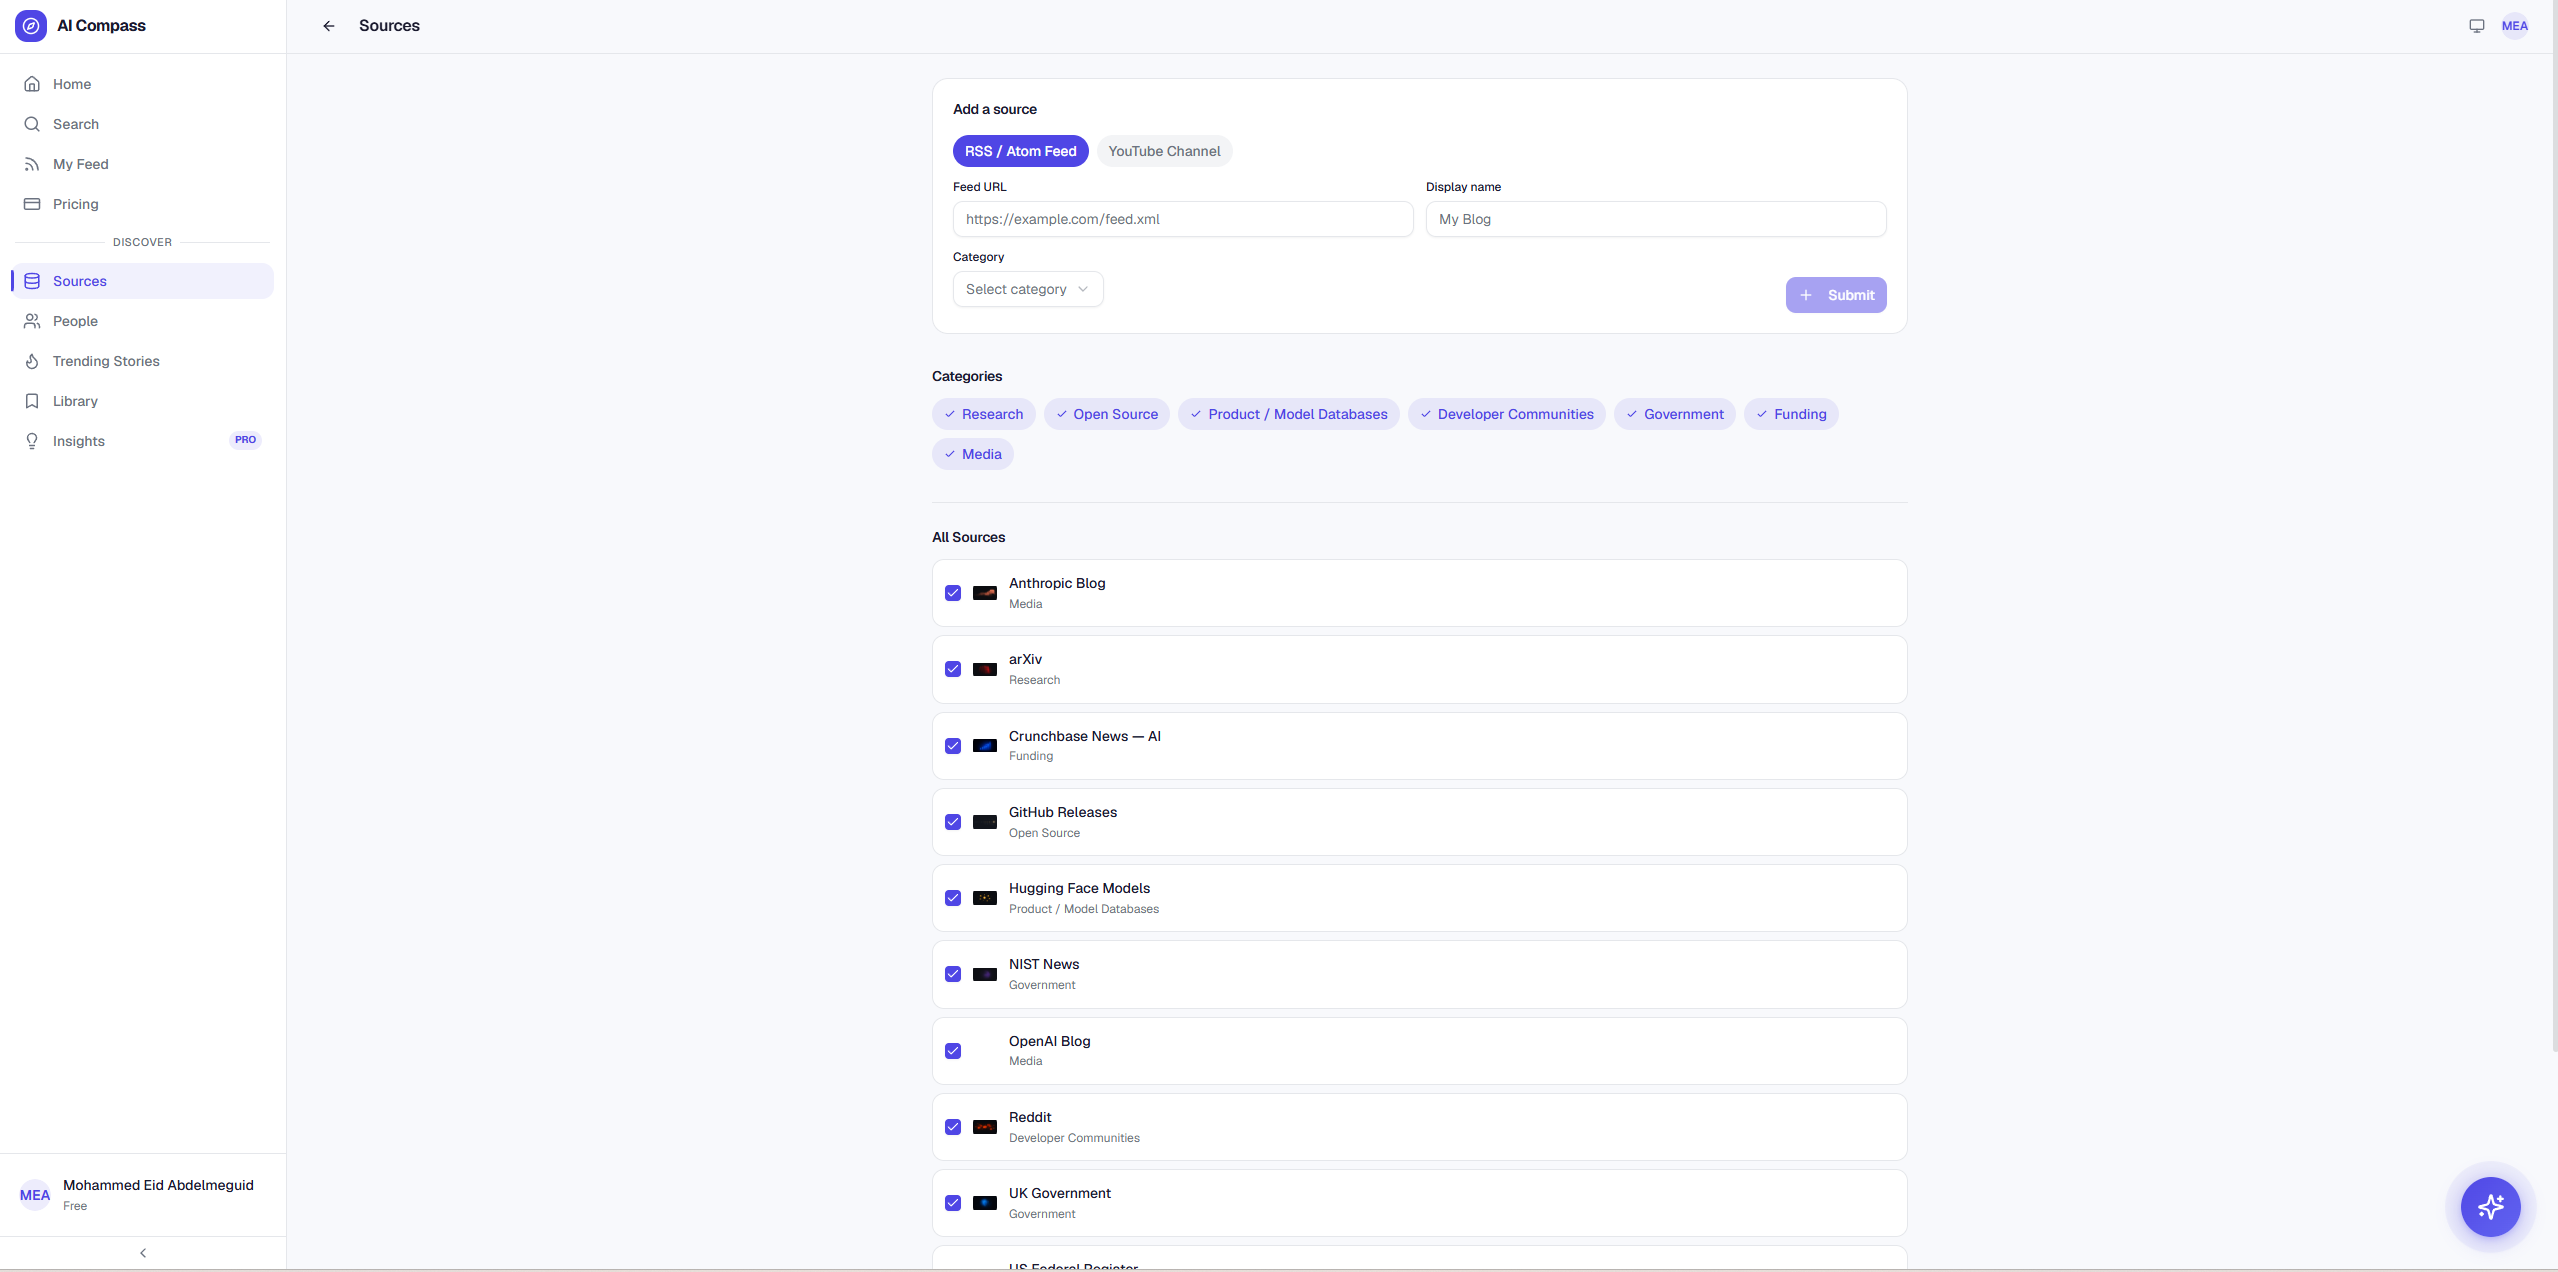
\includegraphics[width=0.85\textwidth]{figures/screenshots/screenshot_sources.png}
\caption{The Sources page, listing the registry-dispatched sources of Table~\ref{tab:sources} with per-user visibility toggles, category filters, and the submission form feeding the relevance gate (Section~\ref{sec:relevance-gate}).}
\label{fig:screenshot-sources}
\end{figure}
